%
\documentclass[fleqn]{jreport}%<--- class はjreport
\usepackage{sotsuron}         %<----- 修論、卒論用のスタイルファイル
\usepackage{ascmac}
\usepackage[dvipdfmx]{graphicx}
%\usepackage{graphicx,psfrag}
\usepackage{epsf}
%\usepackage{fracdull}
\renewcommand{\labelenumi}{[\theenumi]}

%$$$$$$$$$$$$$$$$$$$$$$$$$$$$$ YNU report paper size $$$$$$$$$$$$$$$$$$$$$$
\topmargin -15mm %ORG 
\oddsidemargin -0.1in %ORG 
\evensidemargin -0.1in %ORG 
\baselineskip 7.833mm %ORG 
\textheight 25.2cm %ORG
%\textheight 23.0cm
\textwidth 17cm %ORG
%$$$$$$$$$$$$$$$$$$$$$$必ず次の4つは必要$$$$$$$$$$$$$$$$$$$$$$
\renewcommand{\bf}{\bfseries}
\renewcommand{\gt}{\gtfamily}
\renewcommand{\sf}{\sffamily}
\newcommand{\bm}[1]{\mbox{\boldmath $#1$}}
\usepackage{amsmath}
%\renewcommand{\normalsize}{\fontsize{10pt}{12pt}\selectfont}
%$$$$$$$$$$$$$$$$$$$$$$$$$$$$$$$$$$$$$$$$$$$$$$$$$$$$$$$$$$$$$$$$$$$$$$$$$$
\newcommand{\epsf}[1]{\includegraphics{#1}}
%$$$$$$$$$$$$$$$$$$$$$$$$$$$$$$$$$$$$$$$$$$$$$$$$$$$$$$$$$$$$$$$$$$$$$$$$$$
%\def\epsfile#1{\vspace*{3cm}EPFfigure}
%
%\includeonly{equip}
%$$$$$$$$$$$$$$$$$$$$$$$$$$   表 紙   $$$$$$$$$$$$$$$$$$$$$$$$$$$$$$$$$$$$$
%表紙の注意:課題研究報告書には英文は不要
%
\thesis{
  \bf 卒業研究報告書 \\
  \large Graduation Research Report
  }
\title{\bf
  \TeX を用いた卒業研究報告書の書き方 \\
  \normalsize How to Write of Graduation Research Report using \TeX 
  \smallskip
  \large\bf
  }
\professor{
  浅野 洋介\\
  \normalsize Advisory Professor \ Yosuke ASANO 
  }
\date{
  平成17年3月1日提出 \\
  \normalsize March 1, 2005
  }
\author{
  木更津工業高等専門学校 電気電子工学科 \\     
  \normalsize Department of Electrical and Electric Engineering, 
   Kisarazu National College of Technology \\
   \vspace*{5mm}
  95-201 \\
  浅野 洋介\\
  \normalsize Yosuke ASANO
  }
%$$$$$$$$$$$$$$$$$$$$$$$$$$$$$$$$$$$$$$$$$$$$$$$$$$$$$$$$$$$$$$$$$$$$$$$$$$
%%\input{starstyj}
\begin{document}
\maketitle
\maegaki         %ここから要約
% !TEX root = research_report.tex
%上の記述は消さないこと.章(分割ファイル)を増やしたときも忘れずに記述する.
\chapter*{概要}
\thispagestyle{empty}

報告書の概要を書く.1ページ以内に収まるようにすること.

概要は報告書の全ての内容を考慮してまとめること.必然的に一番最後に書くことになる.

\maetsuke        %ここから目次
\tableofcontents %目次
\listoffigures   %図目次
\listoftables    %表目次
\hombun          %ここから本文
% !TEX root = research_report.tex
%上の記述は消さないこと.章(分割ファイル)を増やしたときも忘れずに記述する.
\chapter{序論}

\section{研究背景}

研究背景や研究目的などを書く.自分の研究が研究分野のどこに位置づけられているのか,また,他の関
連研究と比較してどこ点が優れているかを詳しく書く.参考文献を参照しつつ挙げながら書くとよい.

このように参照番号をつける\cite{asimo}

\section{研究目的}

本研究では・・・
% !TEX root = research_report.tex
%上の記述は消さないこと.章(分割ファイル)を増やしたときも忘れずに記述する.
\chapter{理論}
ここの部分にはこの章の概要を記述する.

\section{○○制御理論}

ありがちなのが段落の作り忘れ.以下のように空行を入れると自動的に段落が作成される.

テストテストテストテストテストテストテストテストテストテストテストテストテストテストテストテス
トテストテストテストテストテストテストテストテスト



\section{図表の貼り付け}
表を示したときは必ず参照する.表\ref{t1}のように・・・
\begin{table}[htbp]
\caption{表}
\label{t1}
\begin{center}
  \begin{tabular}[tb]{|c|c|c|c|c|c|c|c|c|}
   \hline
  aa & bb& cc & aa & bb& cc & aa & bb& cc \\ \hline
  aa & bb& cc & aa & bb& cc & aa & bb& cc \\ \hline
  aa & bb& cc & aa & bb& cc & aa & bb& cc \\ \hline
  aa & bb& cc & aa & bb& cc & aa & bb& cc  \\ \hline
  aa & bb& cc & aa & bb& cc & aa & bb& cc \\ \hline
 \end{tabular}
\end{center}
\end{table}

報告書では領域をケチらず,図は大きく貼り付けること.そして,貼り付けた図は表と同様に必ず本文中で
参照する.図\ref{amp}に示すように・・・.
\begin{figure}[htbp]
 \begin{center}
  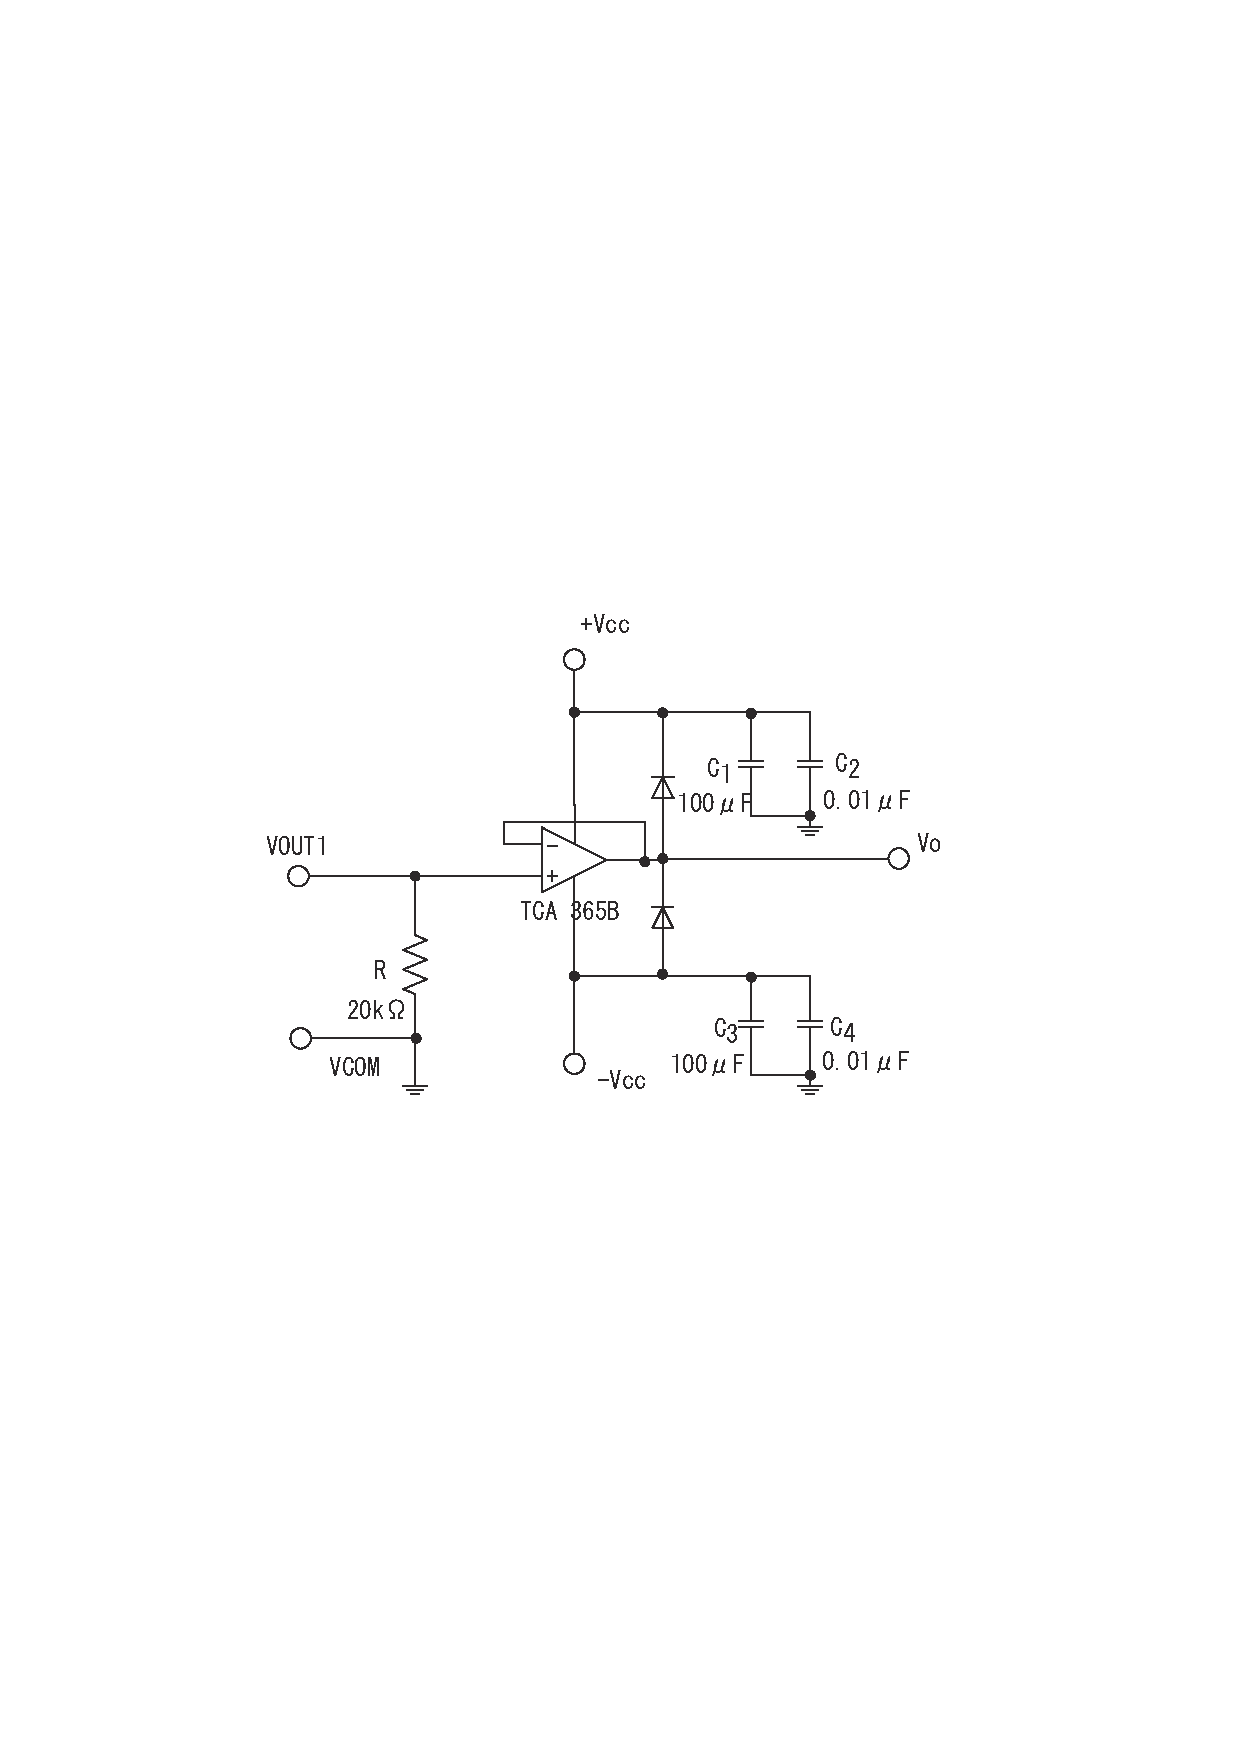
\includegraphics[width = 14.0cm]{./fig/drive_circuit.pdf}
 \end{center}
 \caption{オペアンプ回路図}
 \label{amp}
\end{figure}

これが\TeX のよいところ.図表の位置を変えても自動的に図番号が変化する.

\section{数式}
1行で収まる数式
\begin{equation}
 \int_0^\infty \frac{\sin x}{\sqrt{x}} dx = \sqrt{\frac{\pi}{2}}\label{eq1}
\end{equation}

複数行にわたる数式
\begin{eqnarray}
 \bm{\dot x}&=&\bm{Ax}+\bm{Bu}\label{eq2-1} \\
 \bm{y}&=&\bm{Cx}+\bm{Du}\label{eq2-2}
\end{eqnarray}

文中に数式を入れることも可能$F=m\alpha$である.ただし式番号はつかない.

行列
\begin{equation}
 \begin{bmatrix} 
  A & B & C\\ 
  D & E & F 
 \end{bmatrix}
\end{equation}

ギリシャ文字は数式環境で記述する.\underline{全角で書かない!}

$\alpha,\beta,\gamma,\Gamma,\delta,\Delta,\omega,\Omega,\varepsilon$

必要であれば,式(\ref{eq1}),式(\ref{eq2-1}),式(\ref{eq2-2})のように参照する.

ちなみに,単位はイタリックにしない.$\theta=\frac{\pi}{2}[\mathrm{rad}]$とする.

\include{experiment}
% !TEX root = research_report.tex
%上の記述は消さないこと.章(分割ファイル)を増やしたときも忘れずに記述する.
\chapter{結論}
序論で記述した内容を受けて,研究の結果を集約した物を記述する.なるべく,序論と結論を読んだだけで研究内容がわかるようにするとよい.

結論はあまり長すぎてもよくない.
\shaji          %ここから謝辞
% !TEX root = research_report.tex
%上の記述は消さないこと.章(分割ファイル)を増やしたときも忘れずに記述する.
\chapter*{謝辞}
研究を行なうにあたっての関係者に謝辞を述べる.アドバイスをくれた方,実験機材を貸してくれた方(研究室),研究指導をしてくれた方を洩れないようにすること. 
\bunken         %ここから参考文献
% !TEX root = research_report.tex
%上の記述は消さないこと.章(分割ファイル)を増やしたときも忘れずに記述する.
%\chapter*{参考文献}

\begin{thebibliography}{99}
 \bibitem{asimo}``ASIMO SPECIAL SITE'': http://www.honda.co.jp/ASIMO/
 \bibitem{h6h7} 大学院情報理工学系研究科 知能機械情報学専攻 大学院情報学
	 環・学際情報学府 工学部 機械情報工学科 情報システム工学研究室
	 (JSK)``Perception-Action Integrated Humanoid Robot : H6 \&
	 H7'': http://www.jsk.t.u-tokyo.ac.jp/research/h6/H6\_H7.html
 \bibitem{hrp}独立行政法人産業技術総合研究所 ``Humanoid Robotics Project
	 - 人間協調・共存型ロボットシステム'':
	 http://www.mstc.or.jp/hrp/main.html
 \bibitem{qrio}``SONY Dream Robot QRIO'':
	 http://www.sony.co.jp/SonyInfo/QRIO/index.html
 \bibitem{kawato}``川人学習動態脳プロジェクト'':
	 http://www.kawato.jst.go.jp/DB/home-j.html
 \bibitem{Erbatur} 
	K. Erbatur, A. Okazaki, K. Obiya, T. Takahashi,
	A.Kawamura: ``A Study on the Zero Moment Point Measurement for Biped
	Walking Robots'', Proc. Int. Workshop on Advansed Motion
	 Control, 2002
 \bibitem{hashimoto} 
	橋本 浩一: ``ビジュアルサーボにおける予測と感度'', 計測と制御,
	 Vol. 40, No. 9, pp. 630-635, 2001
 \bibitem{hashimoto2} 
	K. Hasimoto, T. Kimoto, T. Ebine and
	H .Kimura: ``Manipulator Control with Image-Based Visual Servo'',
	IEEE ICRA, pp. 2267--2272, 1991

\end{thebibliography}

書き方は上記のものをまねすること.課題研究では1,2本,卒業研究では10本,専攻科特別研究では20本程
度の論文を読んでおくべきであることから,その本数文の参考文献を挙げる.なるべく,学会誌論文,講演
会論文などを参考文献とするほうがよい.大学内での卒業論文などは入手が困難である確率が高いため載せ
ない方がよい.

本文中で参照した順番に並べること.本文中で参照していないものは最後の方に書く.
 
\appendix       %ここから付録
% !TEX root = research_report.tex
%上の記述は消さないこと.章(分割ファイル)を増やしたときも忘れずに記述する.
\chapter{プログラムソース}

報告書中に書くと論理の流れがおかしくなるものについては付録に記述する.例えば,

\begin{itemize}
 \item ソースコード
 \item 実験機材の詳細な仕様
 \item 詳細な数学的証明 
\end{itemize}

などは付録に載せるべきである.
\end{document}  %おわり

以下は自分用のメモ
abstract.tex               : 要約
introduction.tex           : 序論
robotics.tex               : ロボティクス
conclution.tex             : 結論
thanks.tex                 : 謝辞
reference.tex              : 参考文献
appendix.tex               : 付録









